%% LaTeX2e class for student theses
%% thesis.tex
%% 
%% Karlsruhe Institute of Technology
%% Institute of Information Security and Dependability (KASTEL)
%%
%% Template by
%% Dr.-Ing. Erik Burger
%% burger@kit.edu
%%
%% Adaption by
%% Annika Vielsack
%% vielsack@kit.edu
%%
%% Version 1.0, 2021-07-03

%% Available page modes: oneside, twoside
%% Available languages: english, ngerman
%% Available modes: draft, final (see README)
\documentclass[twoside, english]{afvthesis}
% Copyright 2017 Sergei Tikhomirov, MIT License
% https://github.com/s-tikhomirov/solidity-latex-highlighting/

\usepackage{listings, xcolor}

\definecolor{verylightgray}{rgb}{.97,.97,.97}

\lstdefinelanguage{Solidity}{
	keywords=[1]{anonymous, assembly, assert, balance, break, call, callcode, case, catch, class, constant, continue, constructor, contract, debugger, default, delegatecall, delete, do, else, emit, event, experimental, export, external, false, finally, for, function, gas, if, implements, import, in, indexed, instanceof, interface, internal, is, length, library, log0, log1, log2, log3, log4, memory, modifier, new, payable, pragma, private, protected, public, pure, push, require, return, returns, revert, selfdestruct, send, solidity, storage, struct, suicide, super, switch, then, this, throw, transfer, true, try, typeof, using, value, view, while, with, addmod, ecrecover, keccak256, mulmod, ripemd160, sha256, sha3}, % generic keywords including crypto operations
	keywordstyle=[1]\color{blue}\bfseries,
	keywords=[2]{address, bool, byte, bytes, bytes1, bytes2, bytes3, bytes4, bytes5, bytes6, bytes7, bytes8, bytes9, bytes10, bytes11, bytes12, bytes13, bytes14, bytes15, bytes16, bytes17, bytes18, bytes19, bytes20, bytes21, bytes22, bytes23, bytes24, bytes25, bytes26, bytes27, bytes28, bytes29, bytes30, bytes31, bytes32, enum, int, int8, int16, int24, int32, int40, int48, int56, int64, int72, int80, int88, int96, int104, int112, int120, int128, int136, int144, int152, int160, int168, int176, int184, int192, int200, int208, int216, int224, int232, int240, int248, int256, mapping, string, uint, uint8, uint16, uint24, uint32, uint40, uint48, uint56, uint64, uint72, uint80, uint88, uint96, uint104, uint112, uint120, uint128, uint136, uint144, uint152, uint160, uint168, uint176, uint184, uint192, uint200, uint208, uint216, uint224, uint232, uint240, uint248, uint256, var, void, ether, finney, szabo, wei, days, hours, minutes, seconds, weeks, years},	% types; money and time units
	keywordstyle=[2]\color{teal}\bfseries,
	keywords=[3]{block, blockhash, coinbase, difficulty, gaslimit, number, timestamp, msg, data, gas, sender, sig, value, now, tx, gasprice, origin},	% environment variables
	keywordstyle=[3]\color{violet}\bfseries,
	identifierstyle=\color{black},
	sensitive=false,
	comment=[l]{//},
	morecomment=[s]{/*}{*/},
	commentstyle=\color{gray}\ttfamily,
	stringstyle=\color{red}\ttfamily,
	morestring=[b]',
	morestring=[b]"
}

\lstset{
	language=Solidity,
	backgroundcolor=\color{verylightgray},
	extendedchars=true,
	basicstyle=\footnotesize\ttfamily,
	showstringspaces=false,
	showspaces=false,
	numbers=left,
	numberstyle=\footnotesize,
	numbersep=9pt,
	tabsize=2,
	breaklines=true,
	showtabs=false,
	captionpos=b
}
	
%% ---------------------------------
%% | Information about the thesis  |
%% ---------------------------------

%% Name of the author
\author{Michele Massetti}

%% Title (and possibly subtitle) of the thesis
\title{Security Analysis Tools for Ethereum Smart Contracts: A Comparison Based on Real-World Exploits.}

%% Type of the thesis 
\thesistype{Master's Thesis}

%% Change the institute here, ``KASTEL'' is default
% \myinstitute{Institute of \dots}

%% You can add a grouplogo in the ``logos'' directory.
%% In this case, enable the group logo.
% \showgrouplogo
%% By default it uses the file called grouplogo. But you can choose a different file.
% \grouplogo{myfile}

%% The reviewers are the professors that grade your thesis
\reviewerone{Prof. Bernhard Beckert, Prof. Valentina Gatteschi}

%% If you know who your second reviewer is, add the following line:
% \reviewertwo{Prof. NAME}

%% The advisors are PhDs or Postdocs
\advisorone{Jonas Schiff}
%% The second advisor can be omitted
% \advisortwo{NAME, M.\,Sc.}

%% Please enter the start end end time of your thesis
\editingtime{15 April 2022}{xx MONTH 20XX}

%% The place where you sign the declaratory statement
\signingplace{Karlsruhe}

\settitle

%% --------------------------------
%% | Settings for word separation |
%% --------------------------------

%% Describe separation hints here.
%% For more details, see 
%% http://en.wikibooks.org/wiki/LaTeX/Text_Formatting#Hyphenation
\hyphenation{
% me-ta-mo-del
}

%% --------------------------------
%% | Bibliography                 |
%% --------------------------------

%% Use biber instead of BibTeX, see README
\usepackage[citestyle=authoryear,style=numeric-comp,natbib=true,backend=biber]{biblatex}
\addbibresource{thesis.bib}
\usepackage{listings}
\usepackage{pifont}
\newcommand{\xmark}{\ding{55}}%
\usepackage{amssymb}
\usepackage{pgfgantt}
%% ====================================
%% ====================================
%% ||                                ||
%% || Beginning of the main document ||
%% ||                                ||
%% ====================================
%% ====================================
\begin{document}

%% Set PDF metadata
\setpdf

%% The Preamble begins here
\frontmatter

%% Set the title
\maketitle

%% LaTeX2e class for student theses
%% sections/declaration.tex
%% 
%% Karlsruhe Institute of Technology
%% Institute of Information Security and Dependability (KASTEL)
%%
%% Template by
%% Dr.-Ing. Erik Burger
%% burger@kit.edu
%%
%% Adaption by
%% Annika Vielsack
%% vielsack@kit.edu
%%
%% Version 1.0, 2021-07-03


%% The German text is taken from §14(5) in
%% https://www.informatik.kit.edu/downloads/info%20bsc%20spo%202015.pdf

\thispagestyle{empty}
\null\vfill
 \noindent%
%\hbox to \textwidth{\hrulefill}%
\iflanguage{english}{%
  I hereby declare that the work presented in this thesis is entirely
  my own. I confirm that I specified all employed auxiliary resources
  and clearly acknowledged anything taken verbatim or with changes
  from other sources. I further declare that I prepared this thesis in
  accordance with the rules for safeguarding good scientific practice
  at Karlsruhe Institute of Technology (KIT).}{%
  Ich versichere wahrheitsgemäß, die Arbeit selbstständig verfasst,
  alle benutzten Hilfsmittel vollständig und genau angegeben und alles
  kenntlich gemacht zu haben, was aus Arbeiten anderer unverändert
  oder mit Änderungen entnommen wurde, sowie die Satzung des KIT zur
  Sicherung guter wissenschaftlicher Praxis beachtet zu haben.}

 
%% ---------------------------------------------
\bigskip\noindent
\thesigningplace, \theeditend
\vspace{1.5cm}
 
\noindent\dotfill\hspace*{8.0cm}\\
\hspace*{2cm}(\theauthor) 
\cleardoublepage


%% ----------------
%% |   Abstract   |
%% ----------------
 
%% For theses written in English, an abstract both in English
%% and German is mandatory.
%%
%% For theses written in German, a German abstract is sufficient.
%%
%% The text is included from the following files:
%% - sections/abstract

\includeabstract

%% ------------------------
%% |   Table of Contents  |
%% ------------------------
\tableofcontents

\listoffigures
\listoftables

%% -----------------
%% |   Main part   |
%% -----------------

\mainmatter

%% LaTeX2e class for student theses
%% sections/introduction.tex
%% 
%% Karlsruhe Institute of Technology
%% Institute of Information Security and Dependability (KASTEL)
%%
%% Template by
%% Dr.-Ing. Erik Burger
%% burger@kit.edu
%%
%% Adaption by
%% Annika Vielsack
%% vielsack@kit.edu
%%
%% Version 1.0, 2021-07-03
\chapter{Introduction}
\label{ch:Introduction}


\section{Motivation}
\label{sec:Introduction:Motivation}

Blockchain represents one of the most popular trends in finance and computer science, 
during the last few years the number of investments has been growing exponentially. 
According \citet{CoinGeko}, the crypto market's value is standing around \$2 trillion.

Bitcoin can be considered the “father” of this technology. \citet{Bitcoin} depicted that in his paper, and in the early 2009,
it was effectively launched and the cryptocurrency Bitcoin was introduced. 
\citet{CoinGeko} states the value of Bitcoin around \$38,553.70 and its market capitalization more than  \$700 billions.

Many blockchain systems have been born with new capabilities, 
which have allowed them to fit many different use cases. The first, which allowed developers to 
code on top of itself, was Ethereum.
\citet{Ethereum} published its whitepaper in 2014, and in 2015 it was deployed.
The revolutionary aspect of Ethereum is the introduction of Smart Contract.
These are programs running on blockchain systems and give the developers the opportunity to interact directly 
with this new technology. 
The development of innovative and prominent applications is a consequence of their development, such as NFT marketplaces, music royalty tracking, supply chain and logistics monitoring, voting mechanism, 
cross-border payments, and many others.  

Interest in such a market has grown even among malicious attackers. 
Attacks such as the “Parity Wallet Hack” and the “Decentralized Autonomous Organization Attack” cost millions of dollars simply because of 
naive bugs in the smart contract code. Blockchain and smart contract technologies have multiple aims, but unfortunately, new applications 
based on them still contain bugs and multiple vulnerabilities, which cause 
several issues for the end-users. Most of the use of this technology relates to finance or certifications, therefore integrity, 
authentication and authorisation in transactions are mandatory. The research field behind blockchain technology is growing, as well as the one concerning 
its security and accordingly, many analysis tools were developed. 
These incorporate various strategies for performing the analyses, concerning the technical aspects of smart contracts, 
so these would work differently according to the object of the analysis. 

The topic that will be addressed in this thesis work is the comparison of security analysis tools for smart contracts, based on real-world exploits, so attacks that have happend during the recent years. 
It involves the understanding of smart contracts properties and the usage of different tools, 
providing insight regarding their behaviours in different contexts.

This thesis does not involve well-known benchmarks, with already studied vulnerabilities, 
but the tests are smart contracts involved in attacks. 
Our literature research faced off wide documentation of comparison of tools based on benchmarks and studied vulenrablities, 
but this work's ambition is to verify the effectiveness of the tools in real cases.

\section{Research Goals}
\label{sec:Introduction:ResearchGoals}
The main goal of this thesis can be summerized with the following research question:

\emph{How do state-of-the-art analysis tools for Ethereum/Solidity perform on real-world exploits?}

This thesis involeves eight security analysis tools, which are chosen based on a literature research and on the type of analysis, trying to have a range of different typologies.
Their analysis targets are smart contracts, involved in attacks, which have occured in the last two years (since 2020). 
One of the goals is the definition of the violated properties of those, understanding how they are computed by the attackers.

Furthermore, the comparison of the tools is based on a range of factors, these are some of the parameters used for providing a comparison and an evaluation of the tools.
\begin{itemize}
  \item the performance;
  \item the completeness of the analysis;
  \item the facility of usage, involving the amount of code to be provided;
  \item the amount of found vulnerabilities;
  \item the report interpretability;  
  \item the time for the configuration;
\end{itemize}  

The research question deals with different topics, which can be expressed with the following sub questions: 
\begin{enumerate}
  \item How does a tool perform the analysis? 
  \item Which properties have been violated in the real-world exploits? 
  \item Which vulnerabilities are the tools able to detect? 
  \item In which context a tool perform better?
\end{enumerate}


\section{Releted Works}
\label{sec:Introduction:ReletedWorks}
Nowadays multiple surveys and research work addressing smart contracts analysis have been published. 
The ones, we are interested in, deal with the review of vulnerabilities, description and comparison of tools and definition of new techniques for scanning those. 

The selection of tools was anticipated by research work. 
We picked those starting from surveys and papers, 
regarding comparison of multiple of tools, such as \citet{Survey1}, \citet{Survey2}, \citet{Survey3}, \citet{Survey4}, \citet{thesis}. 
These give a general overview and provide a comparison based on different aspects: type of installation, running mode or type of analysis. 
A taxonomy is provided as well. 
For having a deeper knowledge of every single tool, we considered their papers and documentation.

In this thesis, we involved automated tools (\citet{Slither}, \citet {Mythril}) and the ones which provide the possibility to run custom analysis.
The first ones have as targets vulnerabilities such as reentrancy, overflow/underflow, and gas exceptions; but they do not provide functional correctness guarantees. 
On the other hand, the second group try to solve these issues by providing more possibilities for modelling the analyses. 
We involved tools adopting formal verification (\citet{CertoraDocumentation}, \citet{SolcVerify}, \citet{CelestialPaper}) and fuzzing (\citet{Echidna}). 

The cited works provide a comparison based on well-known benchmarks, defined vulnerabilities or just on the specifications.
This work provides a comparison between the considered tools as well, 
but we tried to move a step forward.
Rather than considering defined vulnerabilities, we consider real-world exploits, which have happened in the last couple of years.

The considered tools are installed and run on real-world attacks; these are chosen based on their effectiveness and the damage, in terms of drawn liquidity.
%% LaTeX2e class for student theses
%% sections/content.tex
%% 
%% Karlsruhe Institute of Technology
%% Institute of Information Security and Dependability (KASTEL)
%%
%% Template by
%% Dr.-Ing. Erik Burger
%% burger@kit.edu
%%
%% Adaption by
%% Annika Vielsack
%% vielsack@kit.edu
%%
%% Version 1.0, 2021-07-03
\definecolor{codegreen}{rgb}{0,0.6,0}
\definecolor{codegray}{rgb}{0.5,0.5,0.5}
\definecolor{codepurple}{rgb}{0.58,0,0.82}
\definecolor{backcolour}{rgb}{0.95,0.95,0.92}

\lstdefinestyle{mystyle}{
    backgroundcolor=\color{backcolour},   
    commentstyle=\color{codegreen},
    keywordstyle=\color{magenta},
    numberstyle=\tiny\color{codegray},
    stringstyle=\color{codepurple},
    basicstyle=\ttfamily\footnotesize,
    breakatwhitespace=false,         
    breaklines=true,                 
    captionpos=b,                    
    keepspaces=true,                 
    numbers=left,                    
    numbersep=5pt,                  
    showspaces=false,                
    showstringspaces=false,
    showtabs=false,                  
    tabsize=2
}

\lstset{style=mystyle}
\chapter{Preliminary Knowledge}
\label{ch:Backgroud}

\section{History}
\label{sec:Backgroud:History}


\section{Bitcoin}
\label{sec:Backgroud:Bitcoin}

\section{Ethereum}
\label{sec:Backgroud:Ethereum}

\section{Smart Contract}
\label{sec:Backgroud:SmartContracts}

\section{Security Analysis}
\label{sec:Backgroud:SecurityAnalysis}



\chapter{Most Common Vulnerabilities}
\label{ch:Vulnerabilities}

Presentation of what effected the smart contrats in the recent year.
The vulnerabilities that I found more often in papers that I read and I selected because I think they are the 
most rappresentative and the most common used by the attackers.

As introduction, I cite some papers that I read dealing with this topic. I select the following vulnerabilities, because I think they represent a risk still today.

\section{Race Codition}
\label{sec:Vulnerabilities:RaceCondition}
Race condition represents in computer science one of the most common vulnerabilities.
\citet{RaceConditionDef} identifies this as an even,  which occurs when two threads access a shared variable at the same time.
A case is illustruted when two threads read the value of a shared variable. After computing operations on that, they update the shared variable. The change applied by the last thread will be preserved and the other one will be lost.
In a Solidity context an analogous situation can happen. This can be exploited by attackers, for withrowing a higher amount of token or manipulating the price of it.

\citetitle{NotSoSmartContracts} is a repository that contains examples of common Ethereum smart contract vulnerabilities.
Vulnerable smart contracts and explanations are coupled and presented. I considered the smart contract \href{https://github.com/crytic/not-so-smart-contracts/blob/master/race_condition/RaceCondition.sol}{RaceCodition.sol} for showing a case of this class of vulnerability.
The vulnerability relies on the shared variable price, which is updated by the function changePrice (\autoref{lst:RaceCodition} line 15) and used by the function buy (\autoref{lst:RaceCodition} line 2).
\begin{lstlisting} [language={Solidity},caption={Cross-function RaceCondition vulnerable functions.}, label={lst:RaceCodition}]

    function buy(uint new_price) payable
        public
    {
        require(msg.value >= price);

        // we assume that the RaceCondition contract
        // has enough allowance
        token.transferFrom(msg.sender, owner, price);

        price = new_price;
        owner = msg.sender;
    }

    function changePrice(uint new_price){
        require(msg.sender == owner);
        price = new_price; 
    }    
\end{lstlisting}

When a user tries to buy tokens, the owner can call the function for changing the price of the token, consequently the attacked user will spend more than he expected.
 

\section{Denial Of Services}
\label{sec:Vulnerabilities:DOS}
The article \citet{CloudFareDos} of CloudFare, proposes a definition of denial-of-service (DoS) attack. It is a type of cyber attack in 
which an attacker aims to render a computer or a informatic service (logical or phisical) unavailable to its intended users by interrupting the 
device's normal functioning. 

In Solidity contetext, DoS consists of attacks where 
users can leave the contract inoperable for a small period of time, or in some cases, permanently.
It represents a cathegory of attacks, consequently it is not possible to classify a 
spefic vulnerability or methodology for exploiting a thread.

As an example of this class of attack, I selected the smart contract presented by \citet{Dos1}. 
It allows the user to place a bid to the contract. If it is the highest bid, it 
sends the previous leader the current bid and set the leader to the sender with the new highest bid.
The vulnerability relies on line 12 (\refname{lst:DosContract1}): the require condition is respected if the transaction which refunds the old leader doesn not revert. 
An attacker can exploit this vulnerability, creating a smart contract which cannot receive ether. Then it intacts with the vulnerable contract, becoming the leader.
When the vulnerable tries to refund the attacker one, it will always revert because it cannot receive ether and no one could become the new leader.

\begin{lstlisting} [language={Solidity},caption={Dos Vulnerable Contract.}, label={lst:DosContract1}]
    pragma solidity ^0.8.0;

    /**
     * @title VulnerableContract
     * @dev This contract is vulnerable to a denial of service (DoS) attack
     */
    contract VulnerableContract {
        address payable leader;
        uint256 public highestBid;
    
        function bid() external payable {
            require(msg.value > highestBid);
    
            // Refund the old leader, if it fails then revert
            require(leader.send(highestBid));
    
            leader = payable(msg.sender);
            highestBid = msg.value;
        }
    
        /// Helper function to check leader
        function getLeader() external view returns (address) {
            return leader;
        }
    }
    
\end{lstlisting}

\chapter{Real world Exploits}
\label{ch:Exploits}
Real-wolrd exploits that have happend in the recent years.


\section{Cover Protocol:Infinite Minting Exploit Nets Attacker \$4.4M }
\label{sec:Exploits:CoverProtocol}
On the 28th of December 2020, an exploit was abused on Cover Protocol's shield mining contract. 
The article shows the attackers could steal from project around \$ 4 million. 
The target of the attack was the smart contract \href{https://github.com/CoverProtocol/cover-token-mining/blob/main/contracts/Blacksmith.sol}{Blacksmith.sol}, its bug had the result to mint more rewards to the miner. 

\subsection{Cover Protocol}
\label{sec:CoverProtocol:Presentation}

\citet{CoverProtocol} interviewed Alan, the co-founder of the Cover Protocl. In his article he answers some question about his project, regarding its functionality and road map. 
It was an active protocol on the Ethereum blockchain; the developer deployed version 2,  because of the attack. 
Cover Protocol is a peer-to-peer coverage marketplace that utilizes ERC-20 fungible tokens to allow permissionless and non-KYC coverage. 
It can be described as a coverage provider.
The attack affected the rewards contract, consequently, the token's one even.  
The exploit can be classified under the name of "infinite mint".

\subsection{The exlpoit}
\label{sec:CoverProtocol:Exploit}
The develports's team reported \citep{CoverProtocolPostMortem} the technical analysis of the exploit the day after.
The contract containing the vulnerability is Blacksmith.sol. The core protocol was not affected, 
but the minting contract and the \$COVER token became unusable.
Firstly, the attackers created a new balancer liquidity pool for the target contract. The next step was to deposit token in it and execute the exploit, 
withdrawing funds from the contract thanks to a miscalculation of the rewards.
The bug relies on the misuse of two keywords in solidity: storage and memory. 

\paragraph{Memory} This keyword within Solidity allocates memory for a specific variable. 
In this instance, that variable is scoped to a specific function. 
The memory is cleared once the function has executed.

\paragraph{Storage} On the other hand this keyword within Solidity allows variables to act as a pointer into the storage of data in mappings or data structures. 
Storage data is persistent between function calls and transactions. 

The previous has a similar behave to the Random Access Memory (RAM) on a computing device, the latter stores into the persistent memory.

The vulnerable function is the deposit one.
\begin{lstlisting} [language={Solidity},caption={Deposit function.}, label={lst:coverdeposit}]
    function deposit(address _lpToken, uint256 _amount) external override {
        require(block.timestamp >= START_TIME , "Blacksmith: not started");
        require(_amount > 0, "Blacksmith: amount is 0");
        Pool memory pool = pools[_lpToken];
        require(pool.lastUpdatedAt > 0, "Blacksmith: pool does not exists");
        require(IERC20(_lpToken).balanceOf(msg.sender) >= _amount, "Blacksmith: insufficient balance");
        updatePool(_lpToken);

        Miner storage miner = miners[_lpToken][msg.sender];
        BonusToken memory bonusToken = bonusTokens[_lpToken];
        _claimCoverRewards(pool, miner);
        _claimBonus(bonusToken, miner);

        miner.amount = miner.amount.add(_amount);
        // update writeoff to match current acc rewards/bonus per token
        miner.rewardWriteoff = miner.amount.mul(pool.accRewardsPerToken).div(CAL_MULTIPLIER);
        miner.bonusWriteoff = miner.amount.mul(bonusToken.accBonusPerToken).div(CAL_MULTIPLIER);

        IERC20(_lpToken).safeTransferFrom(msg.sender, address(this), _amount);
        emit Deposit(msg.sender, _lpToken, _amount);
  }
\end{lstlisting}
At line 4 of \autoref{lst:coverdeposit}, the state of the pool is stored in a variable with the keyword memory. 
The function update \autoref{lst:coverupdate} is called, which updates the state of the pool. However, the variable pool, 
existing within the function, remains identical. 
\begin{lstlisting} [language={Solidity},caption={Update function.}, label={lst:coverupdate}]
    function deposit(address _lpToken, uint256 _amount) external override {
        require(block.timestamp >= START_TIME , "Blacksmith: not started");
        require(_amount > 0, "Blacksmith: amount is 0");
        Pool memory pool = pools[_lpToken];
        require(pool.lastUpdatedAt > 0, "Blacksmith: pool does not exists");
        require(IERC20(_lpToken).balanceOf(msg.sender) >= _amount, "Blacksmith: insufficient balance");
        updatePool(_lpToken);

        Miner storage miner = miners[_lpToken][msg.sender];
        BonusToken memory bonusToken = bonusTokens[_lpToken];
        _claimCoverRewards(pool, miner);
        _claimBonus(bonusToken, miner);

        miner.amount = miner.amount.add(_amount);
        // update writeoff to match current acc rewards/bonus per token
        miner.rewardWriteoff = miner.amount.mul(pool.accRewardsPerToken).div(CAL_MULTIPLIER);
        miner.bonusWriteoff = miner.amount.mul(bonusToken.accBonusPerToken).div(CAL_MULTIPLIER);

        IERC20(_lpToken).safeTransferFrom(msg.sender, address(this), _amount);
        emit Deposit(msg.sender, _lpToken, _amount);
  }
\end{lstlisting}

Then, deposit function at line 16 \autoref{lst:coverdeposit} estimates the reward per token updating the value of miner.rewardWriteoff, 
but it uses the wronge value of the parameter of pool.accRewardsPerToken.

Following the vulnerabilty, anyone can obtain an insane amount of minted tokens when they execute the claimRewards(address \_lpToken) function. 
This function, which is used to grab their rewards, ends up calling \_claimCoverRewards(Pool memory pool, Miner memory miner) which references the miner.rewardWriteoff. 
As that variable is much smaller than the actual pool.accRewardsPerToken, the contract results in minting an abundance of tokens.





\section{DeFi platform bZX: \$8M hack from one misplaced line of code}
\label{sec:Exploits:bZX}

\citet{bZxProtocol} explains how this protocl works. 
Anyone can use bZx to create apps that allow lenders, borrowers, and traders to interact with Ethereum based 
decentralised finance protocol.
It is a community-run project,moreover all major protocol changes requiring a community vote. 

Protocols can be deleveloped by bZx procol, an example is Fulcrum. 
It is a powerful DeFi platform for tokenized lending and margin trading. 
iTokens (margin loans) represent the earn holders interest on borrowed funds and pTokens (tokenized margin positions) allow your margin positions to be composable.

Unfortunately, it suffered a couple of attacks in February 2020.
The developrs explained the attackers could drain different currences,219,199.66 LINK, 4,502.70 Ether (ETH), 1,756,351.27 Tether (USDT), 
1,412,048.48 USD Coin (USDC) and 667,988.62 Dai (DAI): a total of \$8 millin in value. 
The arrack depends on a bug based on an incorrect sequence of operations.

The object of the attack was the contract named LoanTokenLogicStandard.
It implements the logic behind the protocol, for managing the borrows, loans and all the functionalities.
Every ERC20 token has a transferFrom() function, which has the aim to transfer the tokens.
Calling this function allowed the attacker to create and transfer an iToken to hitself: his balance could be artificially increased.
The duplicated tokens were then redeemed for their underlying collateral, 
with the hackers now “owning” a much higher percentage of the pool, so the attacker could withdraw the tokens.

The snipped code \autoref{lst:internalTransferFrom} shows the vulnerable function. 
The attacker called the function with the same amount of \_from and \_to. 
Since both addresses refer to the same one, line 27 decreases the balance of the address, but then line 31 increases the same balance. 
The problem relies on the estimating of the amount: it is the sum of the sent token and 
a variable (line 23), which stored the value of the balance before the transacion.

\begin{lstlisting} [language={Solidity},caption={Vulnerable function in LoanTokenLogicStandard contract.}, label={lst:internalTransferFrom}]
contract LoanTokenLogicStandard is AdvancedToken, GasTokenUser {
    using SafeMath for uint256;
    using SignedSafeMath for int256;

    modifier settlesInterest() {
        _settleInterest();
        _;
    }
    ... 
    function _internalTransferFrom(
        address _from,
        address _to,
        uint256 _value,
        uint256 _allowanceAmount)
        internal
        returns (bool)
    {
        if (_allowanceAmount != uint256(-1)) {
            allowed[_from][msg.sender] = _allowanceAmount.sub(_value, "14");
        }
        //Vulnerable lines 
        uint256 _balancesFrom = balances[_from];
        uint256 _balancesTo = balances[_to];

        require(_to != address(0), "15");

        uint256 _balancesFromNew = _balancesFrom
            .sub(_value, "16");
        balances[_from] = _balancesFromNew;

        uint256 _balancesToNew = _balancesTo
            .add(_value);
        balances[_to] = _balancesToNew;

        // handle checkpoint update
        uint256 _currentPrice = tokenPrice();

        _updateCheckpoints(
            _from,
            _balancesFrom,
            _balancesFromNew,
            _currentPrice
        );
        _updateCheckpoints(
            _to,
            _balancesTo,
            _balancesToNew,
            _currentPrice
        );

        emit Transfer(_from, _to, _value);
        return true;
    }
    ... 
\end{lstlisting}

The developers corrected the bug in few days. 
It was enough switching some line of code, in order to avoid the operations of sum and subtraction operate on the same balance. 
The code \autoref{lst:CorrectinternalTransferFrom} presents some differences. The operations regarding the receiver's balance are computed (lines 13-15), then those which deal with the sender's one (16-20).
\begin{lstlisting} [language={Solidity},caption={Corrected bug in LoanTokenLogicStandard contract.}, label={lst:CorrectinternalTransferFrom}]
    function _internalTransferFrom(
        address _from,
        address _to,
        uint256 _value,
        uint256 _allowanceAmount)
        internal
        returns (bool)
    {
        if (_allowanceAmount != uint256(-1)) {
            allowed[_from][msg.sender] = _allowanceAmount.sub(_value, "14");
        }
        require(_to != address(0), "15");
        uint256 _balancesFrom = balances[_from];
        uint256 _balancesFromNew = _balancesFrom
            .sub(_value, "16");
        balances[_from] = _balancesFromNew;
        uint256 _balancesTo = balances[_to];
        uint256 _balancesToNew = _balancesTo
            .add(_value);
        balances[_to] = _balancesToNew;
        // handle checkpoint update
        uint256 _currentPrice = tokenPrice();
        _updateCheckpoints(
            _from,
            _balancesFrom,
            _balancesFromNew,
            _currentPrice
        );
        _updateCheckpoints(
            _to,
            _balancesTo,
            _balancesToNew,
            _currentPrice
        );
        emit Transfer(_from, _to, _value);
        return true;
    }   
\end{lstlisting}


\section{XSURGE on BSC Chain}
\label{sec:Exploits:XSURGE}

The \citet{XSurgeWeb}'s whitepaper provides a presentation of the ecosystem.
It is described as a great DeFi investing idea based on proprietary pricing algorithms embedded in the Surge Token Variants' contracts.
Surge Token Variants each have their own Market Maker, allowing them to trade continuously and outlast both 
centralised and decentralised exchanges. 
The strategy is to reward long-term holding by increasing a
holder's claim of the backing asset. Each Surge Token utilizes a built-in contract exchange system that renounces the need for
a traditional liquidity pool. Both assets are stored within the contract itself, 
rather than a liquidity pool pair of the backing asset to the
token using a traditional market maker method for exchange and price calculation.

One of the Surge Token is SurgeBNB, the one which is my focus of analysis.
\citet{XSurgeBNB} explains in deep how the attack to this contract occured. 
The Official claimed that the attacker had stolen \$5 million in SurgeBNB through a backdoor vulnerability.
XSURGE stated that a potential security vulnerability in the SurgeBNB contract was discovered on August 16th.

The attack is mabe by 4 main steps:
\begin{enumerate}
    \item the attacker borrow  10,000BNB through flash loans.
    \item Use all the BNB to buy SURGE. According to the current price, 
    the attacker can buy 1,896,594,328,449,690 SURGE
    \item He calls the "sell" function, for selling the obtained SURGE.
    \item The sale function alters the data after the transfer, and the transfer code has a reentrance vulnerability.
    When the attack contract acquires BNB, the period before the SURGE contract's state changes 
    (\refname{lst:SellSURGE} line 15 ), the attack contract can use the reentrance 
    vulnerability to purchase SURGE again.
\end{enumerate}

\begin{lstlisting} [language={Solidity},caption={Sell function of Surge (SURGE) token.}, label={lst:SellSURGE}]
    function sell(uint256 tokenAmount) public nonReentrant returns (bool) {
        
        address seller = msg.sender;
        
        // make sure seller has this balance
        require(_balances[seller] >= tokenAmount, 'cannot sell above token amount');
        
        // calculate the sell fee from this transaction
        uint256 tokensToSwap = tokenAmount.mul(sellFee).div(10**2);
        
        // how much BNB are these tokens worth?
        uint256 amountBNB = tokensToSwap.mul(calculatePrice());
        
        // send BNB to Seller
        (bool successful,) = payable(seller).call{value: amountBNB, gas: 40000}(""); 
        if (successful) {
            // subtract full amount from sender
            _balances[seller] = _balances[seller].sub(tokenAmount, 'sender does not have this amount to sell');
            // if successful, remove tokens from supply
            _totalSupply = _totalSupply.sub(tokenAmount);
        } else {
            revert();
        }
        emit Transfer(seller, address(this), tokenAmount);
        return true;
    }
\end{lstlisting}


The bnb Amount of the contract stays intact, and the total amount of SURGE tokens \texttt{ totalSupply }  
has not been updated, because the attack contract spends all of the BNB balance to acquire SURGE
 each time (still remains the quantity before the sell).
As a result, the price of token falls, allowing the attacker to purchase additional SURGE. 


\begin{lstlisting} [language={Solidity},caption={Purchase function of Surge (SURGE) token.}, label={lst:SellPurchase}]
    function purchase(address buyer, uint256 bnbAmount) internal returns (bool) {
        // make sure we don't buy more than the bnb in this contract
        require(bnbAmount <= address(this).balance, 'purchase not included in balance');
        // previous amount of BNB before we received any        
        uint256 prevBNBAmount = (address(this).balance).sub(bnbAmount);
        // if this is the first purchase, use current balance
        prevBNBAmount = prevBNBAmount == 0 ? address(this).balance : prevBNBAmount;
        // find the number of tokens we should mint to keep up with the current price
        uint256 nShouldPurchase = hyperInflatePrice ? _totalSupply.mul(bnbAmount).div(address(this).balance) : _totalSupply.mul(bnbAmount).div(prevBNBAmount);
        // apply our spread to tokens to inflate price relative to total supply
        uint256 tokensToSend = nShouldPurchase.mul(spreadDivisor).div(10**2);
        // revert if under 1
        if (tokensToSend < 1) {
            revert('Must Buy More Than One Surge');
        }
        
        // mint the tokens we need to the buyer
        mint(buyer, tokensToSend);
        emit Transfer(address(this), buyer, tokensToSend);
        return true;
    }
\end{lstlisting}

Repeating three times of Round 2 and Round 3 , the attacker accumulates a large amount of SURGE through reentry, and then sells all the SURGE to make a profit.

At the end of this transaction, the attack contract sold 1,864,120,345,279,610,000 SURGE, 
obtained 10327 BNB, and finally the profitable 297 BNB was sent to the attacker's address.

The following are the modifications suggested by the Beosin technical team for this attack:
\begin{itemize}
    \item any transfer operation should be place after the state changes to avoid reentry assaults.
    \item Instead of using "call. value," use transfer or send to transfer. 
\end{itemize}

\section{CBDAO: an example of rug pull}
\label{sec:Exploits:CBDAO}
Developers should watch out for possible attacks. They should audit and test their contract to find possible vulnerabilities and apply patches.
In the decentralized finance context, even the investors should worry about malicious developers, who convince the investors to invest and then steal their investments.
These class of fraud are basically  type of exit scam and decentralized finance (DeFi) exploit, it is classified with the name of rug pull.


\citet{RugPullDef} defines rug pull as a  type of crypto scam that occurs when a team pumps their project's token before disappearing with the funds, 
leaving their investors with a valueless asset. 
Fraudulent developers create a new crypto token, 
pump up the price and then pull as much value out of them as possible before abandoning them as their price drops to zero.

An example of this type of fraud is the one presented in the article \citet{CBDAO}.
It seems the malicious developers could steal around 1 million dollar in ethereum (ETH). 

The project main token was \$BREE. For attracting ealry investors, they associeted to it a presale token, named \$SBREE. 
The ones who bought that, could swap their amount of presale token in \$BREE once the token was published, having an advantage.
Unfortubatly, one of the admin wallets exploited a backdoor in the SBREE token contract, minted 50,000 SBREE. After that, the attacker soled that amount in BREE token and sold it on the market.
That pushed down the price of BREE at the expense of other holders. The 50,000 BREE was sold for under 200 ETH.

Following the operation of the \href{https://etherscan.io/address/0x85c90f369676789d3234ecf07adb5262df1bcf15#tokentxns}{malicious developer}, it is possible to understand how the fraud occured.
\href{https://etherscan.io/tx/0x3bf7b06d6737e6d222234acc58dea634c7ff75e6cc447bece6cc264f2e1db9d2}{This transacion}, achieved by etherscan, shows the attacker called the mint function and could generate 
50.000 SBREE. After that, it called the \href{https://etherscan.io/address/0x60c3094a586b02cb416ec4df31119d4513ff0dde#code}{BreePurchase} 
contract for swapping the token in BREE and then swap those in ETH on Uniswap.

The backdoor relies on the malicious management of access control. The admin, with the function grantRole, allow another wallet to be the Minter, so it called the function mint.
\begin{lstlisting} [language=Solidity, caption={Backdoor inside the contract}, label={lst:SBREE}]
    
    ... 
    function _grantRole(bytes32 role, address account) private {
        if (_roles[role].members.add(account)) {
            emit RoleGranted(role, account, _msgSender());
        }
    }
    ... 


    contract Roles is AccessControl {

    bytes32 public constant MINTER_ROLE = keccak256("MINTER");
    bytes32 public constant OPERATOR_ROLE = keccak256("OPERATOR");

    constructor () public {
        _setupRole(DEFAULT_ADMIN_ROLE, _msgSender());
        _setupRole(MINTER_ROLE, _msgSender());
        _setupRole(OPERATOR_ROLE, _msgSender());
    }

    modifier onlyMinter() {
        require(hasRole(MINTER_ROLE, _msgSender()), "Roles: caller does not have the MINTER role");
        _;
    }

    modifier onlyOperator() {
        require(hasRole(OPERATOR_ROLE, _msgSender()), "Roles: caller does not have the OPERATOR role");
        _;
    }
}

//the contract inherit Roles contetract
    ... 
    modifier onlyMinter() {
        require(hasRole(MINTER_ROLE, _msgSender()), "Roles: caller does not have the MINTER role");
        _;
    }
    ... 
    function _mint(address account, uint256 amount) internal virtual {
        require(account != address(0), "ERC20: mint to the zero address");

        _beforeTokenTransfer(address(0), account, amount);

        _totalSupply = _totalSupply.add(amount);
        _balances[account] = _balances[account].add(amount);
        emit Transfer(address(0), account, amount);
    }
    ... 


\end{lstlisting} 
    

\chapter{Analysis Tools}
\label{ch:Tools}
In this chapter I describe the tools and their capabilities, how they perform the Analysis.

\section{Typologies of Tools}
\label{sec:Tools:Typologies}
I explain the different types of analysis exsting in general, as Symbolic execution, formal specification, scanner, Symbolic execution.

\section{Tools for analysing properties specified by user}
\label{sec:Tools:Specification}
Description of Different types of tool, like a taxonomy.

Description of tools that we are going to use. 
I would say like an overview of their papaer.

\subsection{Celestial}
\label{sec:Specification:Celestial}


\subsection{SmartPulse}
\label{sec:Specification:SmartPulse}

\subsection{VeriSol}
\label{sec:Specification:VeriSol}


\subsection{Echidna}
\label{sec:Specification:Echidna}
Echidna is an open-source smart contract fuzzer, developed by \citet{Echidna}, which makes it easy to automatically generate tests to detect violations in
assertions and custom properties.
Rather than relying on a fixed set of pre-defined bug oracles to detect vulnerabilities
during fuzzing campaigns, Echidna supports three types of proper-
ties: 
\begin{itemize}
    \item user-defined properties (for property-based testing;
    \item assertion checking;
    \item gas use estimation.
\end{itemize}

Figure \autoref{fig:echdina_architecture} depicts the Echidna architecture as a two-step process: pre-processing and fuzzing.
The tool starts with a collection of contracts that have been supplied, as well as attributes that have been integrated into one of the contracts.
Echidna uses Slither , smart contract static analysis framework presenet in \autoref{sec:WithoutSpecification:Slither}, to build and analyse the contracts in order to find relevant constants and functions that directly handle Ether (ETH).
The fuzzing effort begins in the second stage. 
Using the application binary interface (ABI) given by the contract, significant constants stated in the contract, 
and any previously gathered sets of transactions from the corpus, this iterative procedure creates random transactions. 
When a property violation is detected, a counterexample is created to indicate the smallest and most basic sequence of operations that caused the failure. 

\begin{figure}
    \centering
    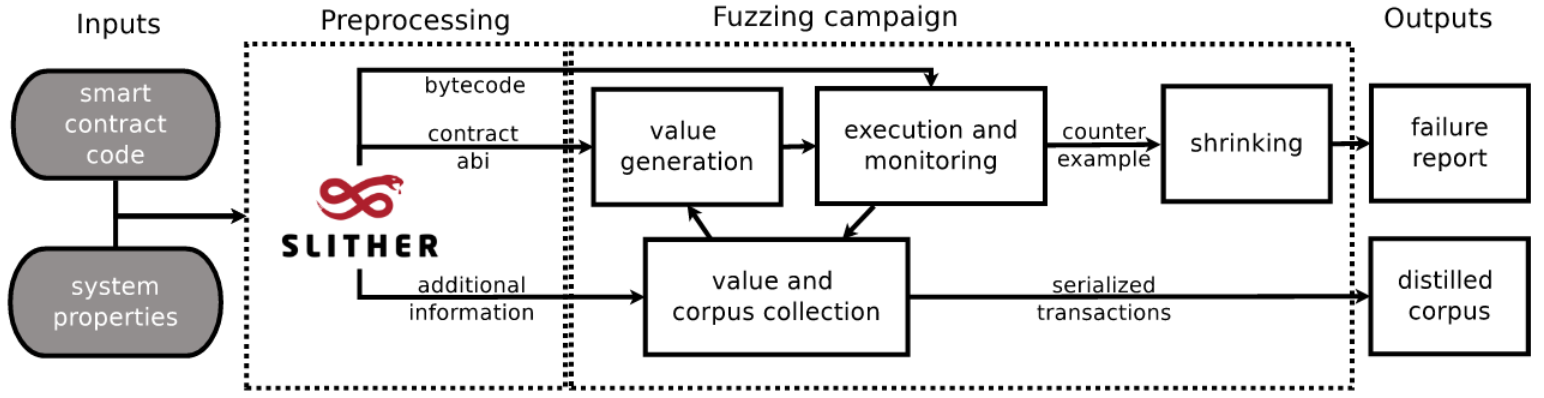
\includegraphics[width=10cm]{logos/echidna.png}
    \caption{Echidna architecture}
    \label{fig:echdina_architecture}
\end{figure}

The code \autoref{lst:EchidnaCode} provides an example of invariant in Echdina context. The Solidity contract contains a vulnerability a the backdoor function. The output of the terminal is presented in Listing \autoref{lst:EchidnaResult}: the attacker. For breaking the property, can call in order the tunctions airdrops() and backdoor()

\begin{lstlisting} [language=Solidity, caption={Solidity smart contract implementing a vulnerable Token and an Echidna invariant function.}, label={lst:EchidnaCode}]
contract Token{
    mapping(address => uint) public balances;
    function airdrop() public{
        balances[msg.sender] = 1000;
    }
    function consume() public{
        require(balances[msg.sender]>0);
        balances[msg.sender] -= 1;
    }
    function backdoor() public{
        balances[msg.sender] += 1;
    }
    function echidna_balance_under_1000() public view returns(bool){
        return balances[msg.sender] <= 1000;
    }
}
\end{lstlisting}
\begin{lstlisting} [caption={Tool's result after the execution of the precious code.}, label={lst:EchidnaResult}]
    $ echidna-test testtoken.sol --contract TestToken
    ...
    echidna_balance_under_1000: failed!
    Call sequence, shrinking (1205/5000):
    airdrop()
    backdoor()

    ...
\end{lstlisting}

The tool can be even used to test assertions. 
The aim is equivalent of the invariant testing methodology, 
but in this case properties are expressed using the Solidity annotation of assertion.

\subsection{Solc-Verify}
\label{sec:Specification:Solc-Verify}

\citet{SolcVerify} present solc-verify, a source-level verification tool for
Ethereum smart contracts. It takes smart contracts written
in Solidity and discharges verification conditions using modular program
analysis. It is built on top of the Solidity compiler, so it reasons at the level of the contract source code. 
Becuase of that, Solc-verify is able to reason about high-level contract attributes 
while accurately modeling low-level language semantics.

Solc-verify is implemented as an extension to the Solidity compiler.
It accepts a collection of Solidity contracts, including specification annotations, and uses 
the Boogie verifier and SMT solvers to discharge verification conditions. 

As \citet{SolcVerify_2} explain, Solc-verify translates the annotated contracts to the Boogie Intermediate Verification
Language (IVL). The key idea of the translation is to encode state variables as global heaps
and functions as procedures. Solc-verify relies on the Boogie verifier to perform modular
verification by discharging verification conditions to SMT solvers. The verification conditions
encode the function body while assuming the preconditions, and then check if postconditions
hold. In this process, function calls are replaced by their specification and loops by their
invariants (modularity). Finally, the results are back-annotated to the Solidity source.

\autoref{lst:SimpleBank} present an example of annotation, which states that the contract will ensure
that the sum of individual balances is equal to the total balance in the bank.


\begin{lstlisting} [language=Solidity, caption={An example Solidity smart contract implementing a simple bank with SolcVerify annotations.}, label={lst:SimpleBank}]
pragma solidity >=0.7.0;

/**
 * @notice invariant __verifier_sum_uint(balances) <= address(this).balance
 */
contract SimpleBank {
    mapping(address=>uint) balances;

    function deposit() public payable {
        balances[msg.sender] += msg.value;
    }

    function withdraw(uint256 amount) public {
        require(balances[msg.sender] > amount);
        bool ok;
        (ok, ) = msg.sender.call{value: amount}(""); // Reentrancy attack
        if (!ok) revert();
        balances[msg.sender] -= amount;
    }
}
\end{lstlisting}




\citet{SolcVerify_3} on GitHub repository, present the specification annotations. Those must be included in special documentation comments (/// or /** */) and must start with the special doctag @notice. 
They must be side-effect free Solidity expressions (with some verifier specific extensions) and can refer to variables within the scope of the annotated element. Functions cannot be called in the annotations, except for getters.
The currently available annotations are listed below. 

\begin{itemize}
    \item Function pre/postconditions can be attached to functions. Preconditions are assumed before executing the function and postconditions are checked (asserted) in the end. The expression can refer to variables in the scope of the function. The postcondition can also refer to the return value if it is named.
    \item Contract level invariants can be attached to contracts. They are included as both a pre- and a postcondition for each public function. The expression can refer to state variables in the contract (and its balance).
    \item Loop invariants can be attached to for and while loops. The expression can refer to variables in scope of the loop, including the loop counter.
    \item Modification specifiers can be attached to functions. The target can be a (1) state variable, including index and member accesses or (2) a balance of an address in scope. Note however, that balance changes due to gas cost or miner rewards are currently not modeled.
    \item Event data specification can be attached to events that should be emitted when certain data changes. 
    Events can declare the state variable(s) they track for changes, or in other words, the variables for which the event should be emitted on a change.
\end{itemize}

\section{Tools without specification}
\label{sec:Tools:WithoutSpecification}

\subsection{VeriSmart}
\label{sec:WithoutSpecification:VeriSmart}

\subsection{SmartTest}
\label{sec:WithoutSpecification:SmartTest}

SmartTest is a safety analayzer for Ethereum smart contracts develeoped by \citet{SmarTest}. 
It adopts a symbolic execution technique for effectively detecting vulnerable transaction sequences. 
The main challenge of the project involves the tool to find transaction sequences,
revealing the vulnerabilities of the analysed smart contract. Therefore, bugs are discoved as the cause of the interaction of multiple transactions.
The purpose of SmartTest is to automatically deliver vulnerable transaction sequences, 
which demostrate the weaknesses of the smart contract.
The main idea is to build a statistical model using known vulnerable transaction sequences and use it to direct symbolic execution toward 
more successfully detecting unknown vulnerabilities. 
Symbolic execution is guided by statistical language models, so it can prioritize transacion sequences which are likely to reveal vulenrablities.
This statregy involves firstly to run unguided symbolic
execution on existing vulnerable contracts, then to learn a probablity distribution over vulnerable transaction sequences.

The tool is implemented as an extension of VeriSmart \autoref{sec:WithoutSpecification:VeriSmart}.
SmartTest is build on top of that, adding its own functionalities:
\begin{itemize}
    \item symbolic execution with a language model.
    \item Symbolic executor for transaction sequences.
    \item Constraint solving optimization.
\end{itemize}
The installation of VeriSmart is necessary for running the tool. After that, the command \autoref{lst:SmarTestRun} is run for using VeriSmart in SmarTest mode.
\begin{lstlisting} [caption={SmarTest Command.}, label={lst:SmarTestRun}]
    ./main.native -input examples/leak_unsafe.sol -mode exploit -exploit_timeout 10
\end{lstlisting}

The report \autoref{lst:SmarTestReport} shows an example of output of SmarTest, which provides the sequence of funtions for exploiting the found bug.
\begin{lstlisting} [caption={SmarTest Example Report.}, label={lst:SmarTestReport}]
    [5] [IO] line 39, (balance[_to] + _value) : disproven, 14.528264s
    1: Example
       {}
       {msg.sender: #x0000000000000000000000000000000000010000,
        msg.value: 0}
    2: approve
       {_spender: #x0000200000000000000000000000000000000000,
        _value: 44365792925664701906080996193724747326645573793336555789802397725137091694592}
       {msg.sender: #x0000000000000000001000000000000000000000,
        msg.value: 0}
    3: mintToken
       {_target: #x0000000000000000001000000000000000000000,
        _amount: 87371285831589357636669861644764241805818792173739087408632338890371299803136}
       {msg.sender: #x0000000000000000000000000000000000010000,
        msg.value: 0}
    4: transferFrom
       {_from: #x0000000000000000001000000000000000000000,
        _to: #x0000000000000000001000000000000000000000,
        _value: 44365787749354941813158155617657849918564739183862151684054205258595743830016}
       {msg.sender: #x0000200000000000000000000000000000000000,
        msg.value: 0}

\end{lstlisting}

The detection of  the following six types of security-critical vulnerabilities are supported by the tool: integer over/underflow, 
assertion violation, division-by-zero, 
ERC20 standard violation, Ether-leaking vulnerability (e.g., 
unauthorized access to transfer), and suicidal vulnerability 
(e.g., unauthorized access to selfdestruct).
In the paper, the authors  focus on just those, without considering vulnerabilities that require analysis of
the interaction of multiple contracts to demonstrate the flaws 
(e.g., reentrancy).





\subsection{Slither}
\label{sec:WithoutSpecification:Slither}
Slither is described by \citet{Slither} as an open-source static analysis framework.
It uses its own intermediate representation, SlithIR, which was created to simplify static analysis of Solidity code. 
Concolic analysis, taint analysis, and control flow checking are involved for detecting a variety
of security vulnerabilities. It is designed to provide
granular information about smart contract code and the flexibility necessary to support many applications.

It is mainly used for:
\begin{itemize}
    \item Automated vulnerability detection: a large variety of
    smart contract bugs can be detected without user inter-
    vention.
    \item Automated optimization detection: Slither detects code
    optimizations that the compiler misses.
    \item Code understanding: printers summarize and display
    contracts' information to aid in the study of the codebase.
    \item Assisted code review: through its API, a user can interact
    with Slither.
\end{itemize}

Slither implements more than twenty bug detectors, regarding reetrancy, Uninitialized variables,
Shadowing and many other. The tool allows the developers to integrate more detectors, therefore it extends Slither's capabilities
to detect more advanced bugs.

\citet{SlitherGitHub} is written in python 3 and it is published on GitHub.
During the installation, I did not find any particular issues.

\subsection{Mythril}
\label{sec:WithoutSpecification:Mythril}
Mythril is a security analysis tool for Ethereum smart contracts. It was introduced by \citet{Mythril}.

The tool  relies on concolic analysis, taint analysis and control flow checking of the EVM bytecode to
prune the search space and to look for values that allow exploiting
vulnerabilities in the smart contract.
It is targeted at finding common vulnerabilities, 
and is not able to discover issues in the business logic of an application. \citet{SWCRegistry}'s taxonomy of vulnerabilities is used by Mythril for classify them. 
Listig \autoref{lst:MythrilOutput} illustrates an example of output of Mythril analysis. 
At the secocond line, there is the reference to the vulnerability classified by SWC Registry with the ID of 110 (Assert Violation).


\begin{lstlisting} [caption={Example of the output of Mythril Analysis.}, label={lst:MythrilOutput}]
==== Exception State ====
SWC ID: 110
Severity: Medium
Contract: Token
Function name: transferArray(address[],uint256[])
PC address: 4385
Estimated Gas Usage: 944 - 6585
An assertion violation was triggered.
It is possible to trigger an assertion violation. Note that Solidity assert() statements should only be used to check invariants. Review the transaction trace generated for this issue and either make sure your program logic is correct, or use require() instead of assert() if your goal is to constrain user inputs or enforce preconditions. Remember to validate inputs from both callers (for instance, via passed arguments) and callees (for instance, via return values).
--------------------
In file: test.sol:309

function transferArray(address[] tos, uint256[] values) public returns (bool) {
        for (uint8 i = 0; i < tos.length; i++) {
            require(transfer(tos[i], values[i]));
        }

        return true;
    }

--------------------

\end{lstlisting}

\subsection{Maian}
\label{sec:WithoutSpecification:Maian}

\subsection{Securify}
\label{sec:WithoutSpecification:Securify}

\subsection{ContractLarva}
\label{sec:WithoutSpecification:ContractLarva}
contractLarva is a runtime verification tool for Solidity contracts. 

\chapter{Results of testing}
\label{ch:Results}

%% LaTeX2e class for student theses
%% sections/evaluation.tex
%% 
%% Karlsruhe Institute of Technology
%% Institute of Information Security and Dependability (KASTEL)
%%
%% Template by
%% Dr.-Ing. Erik Burger
%% burger@kit.edu
%%
%% Adaption by
%% Annika Vielsack
%% vielsack@kit.edu
%%
%% Version 1.0, 2021-07-03

\chapter{Evaluation}
\label{ch:Evaluation}


\begin{table*}
    \footnotesize
    \caption{Results}
    \label{tab:Results}
    \begin{tabular}{ccccl}
    \toprule
     Tools  & Constructive output &  Avg lines of code for test & Avg time (in seconds) \\
      \midrule
        Manticore & List of functions, warning for reentrancy  & 4  &  239,5 \\
        SmartTest & List of Functions, Warnings  & 2,5 &  318  \\
        Celestial & List of unproved tests & 21  &  4  \\
        Echidna & List of functions  & 4  & 20,5 \\
        Certora & List of functions   & 34 &  21  \\ 
        SolcVerify & List of unrproved tests  &  18,5 &  10  \\
        Mythril & List of functions,Warnings  & --  &  221  \\ 
        Slither& Warnings & --  &  3,5  \\ 
    \bottomrule
    \end{tabular}
\end{table*}

\begin{table*}
    
    \caption{Analyses Outocomes:    
    \checkmark: Found vulenrablity, \xmark: False Positive, FN: False Negative, --: Discarded }
    \label{tab:Attacks}
    \begin{tabular}{ccccccccc}
    \toprule
     Tools  & Aku & Cover & BZX & Spartan & Uranium & XSURGE &  BurgerSwap & DirtyDogs\\
      \midrule
      Manticore & \xmark & \xmark & \checkmark & \checkmark & \xmark & \checkmark & \checkmark & \checkmark\\
      SmartTest & \checkmark &   \xmark & \checkmark  & \xmark &\checkmark  & -- & -- & --  \\
      Celestial & \checkmark & -- & \checkmark & \checkmark & \checkmark & -- & -- & --  \\
      Echidna  & \checkmark & \checkmark & \checkmark & \checkmark & \checkmark & -- & -- & -- \\
      Certora & \checkmark & \checkmark & \checkmark & \checkmark & \checkmark & -- & -- & -- \\ 
      SolcVerify & \checkmark & \checkmark & \checkmark & \checkmark & \checkmark & \checkmark & \checkmark  & \checkmark \\
      Slither & FN &\xmark  &\xmark & \xmark & \xmark & \checkmark & \checkmark & \checkmark \\ 
      Mythril  & FN & FN & \xmark &\xmark & \xmark & \checkmark & \checkmark & \checkmark\\
    \bottomrule
    \end{tabular}
\end{table*}

\begin{table*}
    
    \caption{Weaknesses/Limitations}
    \label{tab:Weaknesses}
    \begin{tabular}{cl}
    \toprule
        Tools  &  Limitiations \\
        \midrule
        Manticore & Reentrancy is not dectected by properties property based execution, very slow \\
        SmartTest & Reentrancy is not dectected, the analyses are slow \\
        Celestial & External calls are not considered, keywords storage and memory are not recognized  \\
        Echidna &  Reentrancy is not dectected\\
        Certora & Reentrancy is not dectected\\ 
        SolcVerify & It just gives warning, it does not provide a list of transaction for breaking the given property\\
        Mythril & Just flat contracts are allowed   \\ 
        Slither & Great amount of False negative, due to the fact the scan is based on the grammar \\ 
    \bottomrule
    \end{tabular}
\end{table*}

\begin{table*}
\caption{Strenghts}
    \label{tab:Strenghts}
    \begin{tabular}{cl}
    \toprule
        Tools  &  Strenghts \\
        \midrule
        Manticore & One of the mode cover the properties breaking and the scanner one covers the reentrancy\\
        SmartTest & It allows to set the specific vulenrability to look for  \\
        Celestial & Possibility to use different version of F*  \\
        Echidna &  Possibility to run in multiple modes with different grammar (tests or assertions breaking)\\
        Certora & Implements the library of Openzeppelin, SAS no installation needed \\ 
        SolcVerify & Intuitive specification language based on Annotations, it detects reentrancy\\
        Mythril & It deos not need specification, but still provide list of functions for breaking detected vulnerability  \\ 
        Slither & Easiest installation, fastest tool that we used \\ 
    \bottomrule
    \end{tabular}
\end{table*}

\begin{table*}
    \caption{User Expirience}
    \label{tab:UX}
    \begin{tabular}{ccl}
    \toprule
        Tools  &  User Expirience \\
        \midrule
        Manticore & Possibility to run in 2 modes, properties check and scanner  \\
        SmartTest &  \\
        Celestial & Articulated specification language, running in 2 steps, required multiple dependences \\
        Echidna & Possibility to run in multple modes, but not scanner \\
        Certora & SAS (nothing needed to be installed) \\ 
        SolcVerify & Intuitive specification language made by annotations \\
        Mythril  & Easy installationGood documentation and active community \\ 
        Slither & Easy installation \\   
    \bottomrule
    \end{tabular}
\end{table*}

\begin{table*}
    \caption{Certora results; the time is provided by the sas application}
        \label{tab:CertoraTable}
        \begin{tabular}{ccl}
        \toprule
            Attacks & Line of Code for Specifications & Time of Execution\\
            \midrule
            Aku & 52 & 14 \\ 
            Cover & 31 & 21 \\ 
            BZX & 25  & 18 \\ 
            Spartan & 20  & 25\\ 
            Uranium & 42 & 27  \\ 
            XSURGE &  -- & -- \\  
            BurgerSwap &  -- & --\\ 
            DirtyDogs &  -- & -- \\
        \bottomrule
        \end{tabular}
    \end{table*}
\begin{table*}

\caption{SolcVerify results}
        \label{tab:SolcVerifyTable}
        \begin{tabular}{ccl}
        \toprule
            Attacks & Line of Code for Specifications & Time of Execution (seconds)\\
            \midrule
            Aku & 9 & 4 \\ 
            Cover & 13  & 5 \\ 
            BZX & 17  & 9  \\ 
            Spartan & 25 &  17 \\ 
            Uranium  &  23 & 9 \\ 
            XSURGE & 20 & 10 \\  
            BurgerSwap & 11 & 10  \\ 
            DirtyDogs &  30 &  14\\
        \bottomrule
        \end{tabular}
\end{table*}

\begin{table*}
\caption{Celestial results}
    \label{tab:CelestialTable}
        \begin{tabular}{ccl}
        \toprule
            Attacks & Line of Code for Specifications & Time of Execution\\
            \midrule
            Aku & 22 & 4\\ 
            Cover & --  & -- \\ 
            BZX & 15 & 3\\ 
            Spartan & 29 &  5\\ 
            Uranium & 18 &  5\\ 
            XSURGE &  -- & -- \\  
            BurgerSwap &  -- & --\\ 
            DirtyDogs &  -- & -- \\
        \bottomrule
        \end{tabular}
    \end{table*}

\begin{table*}    
    \caption{Echidna results}
    \label{tab:EchidnaTable}
    \begin{tabular}{ccl}
    \toprule
        Attacks & Line of Code for Specifications & Time of Execution\\
        \midrule
        Aku & 7 & 22 \\ 
        Cover & 5 & 7 \\ 
        BZX & 3 & 33  \\ 
        Spartan & 3 & 17   \\ 
        Uranium & 3 & 24 \\ 
        XSURGE & -- & -- \\  
        BurgerSwap &  -- & --\\ 
        DirtyDogs &  -- & -- \\
    \bottomrule
    \end{tabular}
\end{table*}

\begin{table*}
\caption{Manticore results}
    \label{tab:ManticoreTable}
    \begin{tabular}{ccl}
    \toprule
        Attacks & Line of Code for Specifications & Time of Execution (in seconds)\\
        \midrule
        Aku & 6 & 235  \\ 
        Cover & 5 & 245\\ 
        BZX  & 4 & 228\\ 
        Spartan & 3 & 239 \\ 
        Uranium  & 3 & 250\\ 
        XSURGE & -- & 208\\ 
        BurgerSwap  &  -- & 205 \\ 
        DirtyDogs & -- & 203 \\
    \bottomrule
    \end{tabular}
\end{table*}

\begin{table*}
\caption{SmartTest results}
    \label{tab:SmartTestTable}
    \begin{tabular}{ccl}
    \toprule
        Attacks & Line of Code for Specifications & Time of Execution\\
        \midrule
        Aku & 3 & 320 \\ 
        Cover & 2 & 310\\ 
        BZX  & 4& 320 \\ 
        Spartan &2 & 320\\ 
        Uranium  &4 & 320 \\ 
        XSURGE &  -- & -- \\  
        BurgerSwap &  -- & --\\ 
        DirtyDogs &  -- & -- \\
    \bottomrule
    \end{tabular}
\end{table*}


\section{Outcomes of the Analyses}
%% presenting the outcomes of single analyses, so description of the result 
%% this subsection contains objective data, in the next one I add even my point of view
In this section we list all the tool and we present their single 


\paragraph{Manticore} 
\paragraph{SmartTest}
\paragraph{Celestial}
\paragraph{Echidna}
\paragraph{Certora}
\paragraph{SolcVerify}
\paragraph{Mythril}
\paragraph{Slither}

\section{Weaknesses and Strenghts}
%% What I wrote in the table 
%% I talk even about the installation and the running phase

\section{Tools with Specifications Strategies}
%% General Overview of the strategies 
%% Comperison within the strategies 
%% Personal ideas on their usage, how was the language and so on 
The considered tools cover three main strategies for security analysis: fuzzing, symbolic execution and formal verification. 



The following parametes deal with comparison within this subgroup we want to stess for having a deepen view of the comparison.

\paragraph{Formal verification} 
Formal verification is a very powerful security approach, intending to prove or unproved the given specification. 
This perfectly fits with our research goals, such as the detection of bugs or vulnerabilities in our real-world cases. 

We involved three different tools, implementing this approach, for our purpose. Regarding the results, it is clear that these were executed as fast as or even faster than the other ones. 
Certora is the only one which provides a complete list of functions for breaking the rules, rather than just a warning. 
On the other hand, SolcVerify could detect the vulnerabilities involving external call functions, indeed reentrancy. A powerful aspects of this tool is its possibility to express 
loop invariants, the other ones do not allow it.
Considering the grammar for expressing the specifications, SolcVerify is the one which needs the least amount of lines of code, indeed it involves a notification language; 
I found it very intuitive and fast to write down the specifications.

Celestial architecture encompasses two steps: the translation from celestial file to f* and then its verification. The python script converts the ".cel" in f*, used for the proof or unproof.
The provided file included the smart contract's source code plus the expressed specification. These are statements placed at the beginning of a function, otherwise, it is possible to create a sort of function, 
containing boolean formula, which is called by different specifications function with different parameters, it is useful for expressing the same specification for different purpose.  I consider it the one with more limitations, regarding solidity grammar and reentrancy, 
because it could not detect the reentrancy vunlenaribilities and the Cover protocol attack, because the keywords "storage" and "memory" are rejected. 

Certora is the only tool which is not open-source, for our purpose we adopted its free version.
Its specification language is described by its developers' group as "rule-based". It differs from the other two tools under this aspect, because this way gives more elasticity to the user and defines more specific cases.
The rule is composed of some function calls and it concludes with an assertion or more. The user is allowed to test a specific case, using "require" and the possibility to set up a proper environment. 
The preconditions, in this case, are expressed using the Solidity keyword "require" in the rule.

\paragraph{Different stategies, similar grammar}
We considered two tools with similar grammar but implemented different analysis approaches: Manticore and Echidna. 
In both of the cases, we provided functions containing a boolean formula, which the tools try to break. From the results, 
we noticed that Echidna run faster and it worked for all the cases, but Manticore could cover the reentrancy vulnerabilities thanks to its changing architecture.


\section{Customized and Non-specific Analyses}
%% Stressing the important of the specification for a real world case
%% If used in the right context, they are effective 
The objectives of our analyses were smart contracts involved in real-world exploits. The attackers exploited a specific bug or lack of security in the logic of programs. The specifications allowed the user to express the requirements of the program. These provide a customized analysis, its accuracy is demanded by the developer as well. Our work involved smart contracts with well-known vulnerabilities, but the definition of the properties is an indispensable and complex step.
The tools without specification implement vulnerabilities detectors, which are stated in their paper. They have well-defined limitations, but strengths as well. These detect preconfigured vulnerabilities, so a warning can be run even if we expect that indeed the number of false negatives can be relevant.
An example is Slither, which for every comparison of block time stamp give a warning. 

Our results stress the impossibility of the tools without specification for the detection of specific vulnerabilities, but they could correctly detect the reentrancy cases. 
On the other hand, the ones with specifications had problems in the reentrancy detection. The limitations of some of these involve the external calls. 
SolcVerify was the only tool which could provide the possibility of reentrancy detection. Echidna, as Certora, developers specified the tools  can detect the reetracy, in the case an attack is provided, 
but we think this approch ca be useful for checking a possible attack rather than a detection of a vulnerabilityl.
Manticore underlines this aspect, it could bridge this gap adopting 2 different runnning mode. 


\section{Prova }

\section{Prova2}

%% LaTeX2e class for student theses
%% sections/coclusion.tex
%% 
%% Karlsruhe Institute of Technology
%% Institute of Information Security and Dependability (KASTEL)
%%
%% Template by
%% Dr.-Ing. Erik Burger
%% burger@kit.edu
%%
%% Adaption by
%% Annika Vielsack
%% vielsack@kit.edu
%%
%% Version 1.0, 2021-07-03

\chapter{Conclusion}
\label{ch:Conclusion}
The security of smart contracts is a field which has been growing, 
as the popularity of blockchains and decentralised applications (web3, NFTs...) has been getting more spread.

This work presents the behaviour of analysis tools in a real-world context, 
providing insights into the process of definition of properties, usage of the tools and finding vulnerabilities.
It is addressed to present a possible approach in real situations.

Finally, a comparison of the selected tools is produced.
It deals with multiple aspects of those, starting with the installation and the user experience, involving the performance and effectiveness of the analysis.

The aim is to study the aspects of those in a situation as 
similar as possible to realty. 
The last chapters deal with their behaviour, understanding which approach is more effective. 
Moreover, this work covers even the process of definition of the properties.

This thesis provides the description of each tool, dealing with its performance, stating which typology of them had the best results. 
The involved attacks are presented, stating the properties per each of them. 

Security of smart contracts is fundamental for granting the correct behaviour of a decentralised application, but a limitation is a possibility 
of multiple threats involving the infrastructure of the system itself.
Possible attacks on the blockchain are not covered by this field. 
The network itself could be vulnerable and a user could risk getting the private key of the wallet stolen. 

In this field, the definition of the specifications is fundamental.
The focus of this thesis was on the vulnerable parts, for understanding which vulnerabilities were exploited by the attackers.
Dealing with the reviewed attacks, the way those were computed is known. 
The difficulties dealt with the definition of the properties and the correct usage of the tools. 
Reviewing a smart contract involves the additional task of trying to define all the possible vulnerabilities and writing those in form of specifications, 
for effective results from the tools providing custom analysis.

\section{Outlooks}
Further work can use the same tools, 
but analyse new attacks for evaluating the effectiveness of those tools in new real worlds cases.

New researches can adopt the same approach, involving new attacks and new tools.

It can provide the starting point for a code review, supporting developers 
and security analysts for the choice of tools for their experiments and tests, based on a
given selection criteria.



%% --------------------
%% |   Bibliography   |
%% --------------------

%% Add entry to the table of contents for the bibliography
\printbibliography[heading=bibintoc]

%% ----------------
%% |   Appendix   |
%% ----------------
\appendix
%% LaTeX2e class for student theses
%% sections/appendix.tex
%% 
%% Karlsruhe Institute of Technology
%% Institute of Information Security and Dependability (KASTEL)
%%
%% Template by
%% Dr.-Ing. Erik Burger
%% burger@kit.edu
%%
%% Adaption by
%% Annika Vielsack
%% vielsack@kit.edu
%%
%% Version 1.0, 2021-07-03

\iflanguage{english}
{\chapter{Appendix}}    % english style
{\chapter{Anhang}}      % german style
\label{ch:appendix}


%% -------------------
%% | Example content |
%% -------------------
\section{First Appendix Section}
\label{sec:appendix:FirstSection}
		
\setcounter{figure}{0}
		
\begin{figure} [ht]
  \centering
  \caption{A figure}
  \label{fig:anotherfigure}
\end{figure}


\dots
%% ---------------------
%% | / Example content |
%% ---------------------


\end{document}
